\chapter{Physics Theory}%
\label{ch:theory}

The following chapter outlines the physics theory that informs and guides the
experimental process of searching for new particles or making measurements at
a particle collider. Not only are the physics theories described here useful in
that context but they also provide an almost complete picture of the universe at
certain scales. This chapter was written with the aid of notes taken at the
annual STFC High Energy Physics Summer School, and with the aid of several
books~\cite{halzen, thomson_2013}, in which a more detailed description of the
theories can be found.

The Standard Model of particle physics is a theoretical framework that describes
all elementary particles and three of the fundamental forces of nature. Notably
the only force that is not described by the theory is gravity. Particles
described by the model are listed in table~\ref{tab:sm} with a white gap
separating the matter particles (fermions) from the force carrying particles
(bosons). Fermions, which make up solid matter obey Fermi-Dirac
statistics~\cite{Fermi-stat, Dirac-stat} whereas bosons obey Bose-Einstein
statistics~\cite{Bose-Einstein}. The Higgs boson is special in that as far as we
know it does not carry a force in the conventional sense, instead it is
responsible for giving fundamental particles mass, discussed in more detail in
section~\ref{sec:higgs-mech}. In the table of particles quarks (blue) and
leptons (red) are ordered in columns by increasing mass, apart from the
neutrinos, which are massless in the theory.

\begin{table}[ht]
  \centering
  \begin{tikzpicture}[x=1.2cm, y=1.2cm]
  \draw[round] (-0.5,0.5) rectangle (4.4,-1.5);
  \draw[round] (-0.6,0.6) rectangle (5.0,-2.5);
  \draw[round] (-0.7,0.7) rectangle (5.6,-3.5);

  \node at(0, 0)   {\particle[gray!20!white]
                   {$u$}        {up}       {$2.3$ MeV}{1/2}{$2/3$}{R/G/B}};
  \node at(0,-1)   {\particle[gray!20!white]
                   {$d$}        {down}    {$4.8$ MeV}{1/2}{$-1/3$}{R/G/B}};
  \node at(0,-2)   {\particle[gray!20!white]
                   {$e$}        {electron}       {$511$ keV}{1/2}{$-1$}{}};
  \node at(0,-3)   {\particle[gray!20!white]
                   {$\nu_e$}    {$e$ neutrino}         {$<2$ eV}{1/2}{}{}};
  \node at(1, 0)   {\particle
                   {$c$}        {charm}   {$1.28$ GeV}{1/2}{$2/3$}{R/G/B}};
  \node at(1,-1)   {\particle 
                   {$s$}        {strange}  {$95$ MeV}{1/2}{$-1/3$}{R/G/B}};
  \node at(1,-2)   {\particle
                   {$\mu$}      {muon}         {$105.7$ MeV}{1/2}{$-1$}{}};
  \node at(1,-3)   {\particle
                   {$\nu_\mu$}  {$\mu$ neutrino}    {$<190$ keV}{1/2}{}{}};
  \node at(2, 0)   {\particle
                   {$t$}        {top}    {$173.2$ GeV}{1/2}{$2/3$}{R/G/B}};
  \node at(2,-1)   {\particle
                   {$b$}        {bottom}  {$4.7$ GeV}{1/2}{$-1/3$}{R/G/B}};
  \node at(2,-2)   {\particle
                   {$\tau$}     {tau}          {$1.777$ GeV}{1/2}{$-1$}{}};
  \node at(2,-3)   {\particle
                   {$\nu_\tau$} {$\tau$ neutrino}  {$<18.2$ MeV}{1/2}{}{}};
  \node at(3,-3)   {\particle[orange!20!white]
                   {$W^{\hspace{-.3ex}\scalebox{.5}{$\pm$}}$}
                                {}              {$80.4$ GeV}{1}{$\pm1$}{}};
  \node at(4,-3)   {\particle[orange!20!white]
                   {$Z$}        {}                    {$91.2$ GeV}{1}{}{}};
  \node at(3.5,-2) {\particle[green!50!black!20]
                   {$\gamma$}   {photon}                        {}{1}{}{}};
  \node at(3.5,-1) {\particle[purple!20!white]
                   {$g$}        {gluon}                    {}{1}{}{color}};
  \node at(5,0)    {\particle[gray!50!white]
                   {$H$}        {Higgs}              {$125.1$ GeV}{0}{}{}};
  \node at(6.1,-3) {\particle
                   {}           {graviton}                       {}{}{}{}};

  \node at(4.25,-0.5) [force]      {strong nuclear force (color)};
  \node at(4.85,-1.5) [force]    {electromagnetic force (charge)};
  \node at(5.45,-2.4) [force] {weak nuclear force (weak isospin)};
  \node at(6.75,-2.5) [force]        {gravitational force (mass)};

  \draw [<-] (2.5,0.3)   -- (2.7,0.3)          node [legend] {charge};
  \draw [<-] (2.5,0.15)  -- (2.7,0.15)         node [legend] {colors};
  \draw [<-] (2.05,0.25) -- (2.3,0) -- (2.7,0) node [legend]   {mass};
  \draw [<-] (2.5,-0.3)  -- (2.7,-0.3)         node [legend]   {spin};

  \draw [mbrace] (-0.8,0.5)  -- (-0.8,-1.5)
                 node[leftlabel] {6 quarks\\(+6 anti-quarks)};
  \draw [mbrace] (-0.8,-1.5) -- (-0.8,-3.5)
                 node[leftlabel] {6 leptons\\(+6 anti-leptons)};
  \draw [mbrace] (-0.5,-3.6) -- (2.5,-3.6)
                 node[bottomlabel]
                 {12 fermions\\(+12 anti-fermions)\\increasing mass $\to$};
  \draw [mbrace] (2.5,-3.6) -- (5.5,-3.6)
                 node[bottomlabel] {5 bosons\\(+1 opposite charge $W$)};

  \draw [brace] (-0.5,.8) -- (0.5,.8) node[toplabel]         {standard matter};
  \draw [brace] (0.5,.8)  -- (2.5,.8) node[toplabel]         {unstable matter};
  \draw [brace] (2.5,.8)  -- (4.5,.8) node[toplabel]          {force carriers};
  \draw [brace] (4.5,.8)  -- (5.5,.8) node[toplabel]       {Goldstone\\bosons};
  \draw [brace] (5.5,.8)  -- (7,.8)   node[toplabel] {outside\\standard model};

  \node at (0,1.2)   [generation] {1\tiny st};
  \node at (1,1.2)   [generation] {2\tiny nd};
  \node at (2,1.2)   [generation] {3\tiny rd};
  \node at (2.8,1.2) [generation] {\tiny generation};
\end{tikzpicture}
  % \begin{tabular}{|c|c|c|c|c|c|c|}
  %   %\multicolumn{6}{c}{\textbf{Particles of the Standard Model}}
  %   %\\
  %   \hhline{---|~|--}
  %   \cellcolor{blue!18} $u$ &
  %   \cellcolor{blue!18} $c$ &
  %   \cellcolor{blue!18} $t$ &
  %   ~ &
  %   \cellcolor{yellow!18} $g$ &
  %   \cellcolor{green!18} $H$
  %   \\
  %   \cellcolor{blue!18} \small{$up~quark$} &
  %   \cellcolor{blue!18} \small{$charm~quark$} &
  %   \cellcolor{blue!18} \small{$top~quark$} &
  %   ~ &
  %   \cellcolor{yellow!18} \small{$gluon$} &
  %   \cellcolor{green!18} \small{$Higgs$}
  %   \\
  %   \cline{1-3}
  %   \cline{5-6}
  %   %\hhline{~~~~~-}
  %   %\hhline{~~~~~|--|}
  %   \cellcolor{blue!18} $d$ &
  %   \cellcolor{blue!18} $s$ &
  %   \cellcolor{blue!18} $b$ &
  %   ~ &
  %   \cellcolor{yellow!18} $\gamma$
  %   \\
  %   \cellcolor{blue!18} \small{$down~quark$} &
  %   \cellcolor{blue!18} \small{$strange~quark$} &
  %   \cellcolor{blue!18} \small{$bottom~quark$} &
  %   ~ &
  %   \cellcolor{yellow!18} \small{$photon$}
  %   \\
  %   \hhline{---~|-|~}
  %   %\hline
  %   \cellcolor{red!18} $e^-$ &
  %   \cellcolor{red!18} $\mu^{-}$ &
  %   \cellcolor{red!18} $\tau^-$ &
  %   ~ &
  %   \cellcolor{yellow!18} $Z^0$
  %   \\
  %   \cellcolor{red!18} \small{$electron$} &
  %   \cellcolor{red!18} \small{$muon$} &
  %   \cellcolor{red!18} \small{$tau$} &
  %   ~ &
  %   \cellcolor{yellow!18} \small{$Z~boson$}
  %   \\
  %   \cline{1-3}
  %   \cline{5-5}
  %   \cellcolor{red!18} $\nu_{e}$ &
  %   \cellcolor{red!18} $\nu_{\mu}$ &
  %   \cellcolor{red!18} $\nu_{\tau}$ &
  %   ~ &
  %   \cellcolor{yellow!18} $W^\pm$
  %   \\
  %   \cellcolor{red!18} \small{$electron~neutrino$} &
  %   \cellcolor{red!18} \small{$muon~neutrino$} &
  %   \cellcolor{red!18} \small{$tau~neutrino$} &
  %   ~ &
  %   \cellcolor{yellow!18} \small{$W~boson$}
  %   \\
  %   \cline{1-3}
  %   \cline{5-5}
  % \end{tabular}
  \caption{The particles of the standard model with fermions displayed on the
    left and bosons on the right. Quarks are in blue, leptons in red, vector
    bosons in yellow and scalar bosons in green.}
  \label{tab:sm}
\end{table}


As mentioned the model describes forces as being mediated by certain particles,
the photon ($\gamma$) mediates the electromagnetic force, particles experiencing
electromagnetic repulsion or attraction are described as exchanging photons. The
strength and direction of the force experienced is proportional to the
electromagnetic charge of particles involved. The Standard Model is a theory of
quantum fields in which the strength of interactions between fields, or
particles which are described as excitations in the fields, is parametrised by
something known as a coupling constant. It is natural to assume that the
strength of the interaction between photons and charged particles is related to
the electromagnetic charge of the particles involved. Indeed this is the case
consider the Coulomb force between two protons,
\begin{equation}
  F = \frac{e^2}{4\pi\epsilon_0r},
\end{equation}
where $e$ is the elementary charge, $\epsilon_0$ is the electric constant and
$r$ is the distance between the two protons in question and also the
energy of a photon given by
\begin{equation}
  E = \frac{hc}{\lambda},
\end{equation}
where $h$ is Planck's constant, $c$ is the speed of light and $\lambda$ is the
wavelength of the photon. The value of the ratio of these two quantities
\begin{equation}
  \label{eq:fine-structure}
  \alpha = \frac{e^{2}\lambda}{4\pi\epsilon_{0}rhc},
\end{equation}
known as the fine structure constant, is the coupling constant that describes
the strength of the interactions between the photon field and fields of
particles with electromagnetic charge. So as is now clear this coupling constant
does indeed depend on the electromagnetic charge of the objects involved and so
it is not in fact constant.

As well as the electromagnetic force the Standard Model describes the strong
nuclear force and the weak nuclear force, shortened to just the strong and weak
forces respectively. Like the electromagnetic force they too are mediated by the
exchange of particles, the gluons ($g$) carry the strong force and the $W^\pm$
and $Z^0$ bosons carry the weak force.

The charge associated with the strong force is known as colour which can take
values that are mapped onto colours in the visible spectrum (red, green, blue)
for ease of description. For each of these colours an anti-colour is also
allowed (anti-red, anti-green, anti-blue). Unlike with the electromagnetic
charge, particles with colour charge are not found freely in nature. Instead we
find particles known as hadrons which are bound states of quarks and anti-quarks
(e.g. the proton). The phenomenon of coloured particles being bound in such a
manner is known as colour confinement, and the bound states are described by the
quantum numbers isospin ($I$) and hypercharge ($Y_c$). It is commonly assumed
that all free particles in nature are colour singlets e.g. for a hadron the
state could be written as
\begin{equation}
  \label{eq:hadron-colour}
  \frac{(r\bar{r} + b\bar{b} + g\bar{g})}{\sqrt{3}},
\end{equation}
where $r$, $b$ and $g$ represent red, blue and green charges respectively. This
phenomenon is known as quark confinement. Gluons carry colour and anti-colour
indicating that there should be nine possible quantum mechanical states for the
gluon given the available number of colour/anti-colour combinations, however
when one considers that the strong force is exclusively short range, and
therefore that there should be no free gluons (disallowing colour singlet
gluons) the number of possible states is reduced to eight. The state of a
particle, as far as its description with respect to the strong force is
concerned, is given by a vector which lives in a vector space, in which elements
of the Lie group $SU(3)_C$ act as unitary operators, where the $C$ denotes that
the group is associated with the colour charge. The $SU(3)$ group is the group
of $3~\times~3$ unitary matrices whose determinant is one. These correspond to
the eight generators of $SU(3)$ where in general for a group $SU(N)$ the number
of generators is given by $N^2 - 1$.

Describing the weak force requires introducing further quantum numbers weak
isospin $T$ and weak hypercharge $Y_W$. The state of a particle with regards to
the weak force is given by a vector which lives in a vector space in which
elements of $SU(2)_L \times $U(1)$_{Y_{W}}$ act as unitary operators where the
$L$ denotes that only particles in left-handed chiral states interact with the
weak force~\footnote{More specifically only left-handed chiral particles
  participate in weak charged current interactions.}. Left-handed fermions are
represented as doublets in the theory with weak isospin $T = 1/2$ whilst
right-handed fermions are singlets with weak isospin $T = 0$.

Along the way we have described particle states with respect to particular
forces as vectors living in some vector space where the action of the element of
a group has been as a unitary operator. If we are to describe a particle state
taking into account the full model, the group whose elements should act as
unitary operators on the particle state (the gauge group) is $SU{(3)}_{C} \times
SU{(2)}_{L} \times U{(1)}_{Y_{W}}$. For each of the groups in the direct product
we have established a (gauge) symmetry and therefore due to Noether's
theorem~\cite{Noether_1971} there should be an associated conserved quantity.
The conserved quantities in this case are the electric charge, the weak
hypercharge and isospin and the colour charge.


\section{Historical Aside}%
\label{sec:history}

This section provides some historical context surrounding the Dirac equation
which will later be used as the starting point in the discussion of quantum
electrodynamics, which is the sector of the Standard Model that describes
electromagnetic interactions.

In 1905 Albert Einstein first proposed the idea of special
relativity~\cite{Einstein:special}. The aim of the idea was to unify the then
inconsistent theories of Maxwell's electromagnetism and Newtonian mechanics. The
result of Einstein's work was a theory of motion which agreed with the
predictions of Newtonian mechanics at velocities much smaller than the speed of
light but whose predictions were accurate also at much higher velocities (for
which Newtonian predictions fail). Arguably, the most far reaching consequence of
special relativity is that it demands that any equation of motion must be
invariant under Lorentz transformations, at least in terms of the formulation of
new theories is concerned. Many physical phenomena predicted by special
relativity could be considered of higher consequence in general, for example the
phenomena of length contraction, time dilation, energy-mass equivalence and the
universal speed limit (equal to the speed of light in vacuum), all of which are
extensively scrutinised experimentally ~\cite{sr-tests-1, sr-tests-2,
  sr-tests-3, sr-tests-4, sr-tests-5, sr-tests-6, sr-tests-7}. It is the Lorentz
transformation however that should be kept in mind for the following discussion,
the transformation may be written as
\begin{equation}
  \begin{split}
    \begin{aligned}[t]
      &t'&=&\;\;\;\gamma(t -vx/c^{2})\\
      &x'&=&\;\;\;\gamma(x - vt)\\
      \text{with } &\gamma&=&\;\;\;\frac{1}{\sqrt{1 - v^{2}/c^{2}}},
    \end{aligned}
  \end{split}
  \label{eq:lorentz-transform}
\end{equation}
in a single dimension of space $x$ and one of time $t$ where $v$ represents the
velocity of the system described by the primed coordinates relative to the
unprimed coordinates and $c$ is the speed of light in vacuum.  

Twenty years after Einstein introduced the ideas of special relativity Erwin
Schr\"odinger postulated new ideas regarding the motion of quantum mechanical
systems~\cite{Schrodinger}. Though he knew his new equation was not invariant
under Lorentz transformations, and therefore incomplete, Schr\"odinger's
formulation of quantum mechanics changed the way physicists thought about the
universe for ever. His famous equation
\begin{equation}
  \label{eq:schrodinger}
  i\hbar\frac{\partial}{\partial t}\Psi(\vec{x}, t) =
  \Bigg(\frac{-\hbar^{2}}{2m}\nabla^{2} + V(\vec{x}, t)  \Bigg)\Psi(\vec{x}, t),
\end{equation}
describes the states of particles as wave-functions $\Psi$ which can only be
interpreted in a probabilistic manner and contains Planck's constant the quantum
of action. This work had many consequences including the quantisation of the
values of measured observables (meaning they can only take discrete values) and
the descriptions of particles as waves.

It was the aim of Paul Dirac to make the Schr\"odinger equation Lorentz
invariant and thus provide a more complete description of quantum systems. Along
the way he came to the realisation that in order for his equation to satisfy his
needs the wave-function had to be replaced with a four component spinor ($\psi$)
and the introduction of matrices known now as the Dirac matrices (labeled
$\gamma^{\mu} \text{ with } \mu=0,1,2,4$) was required. Though not the form he
originally wrote down Dirac's Lagrangian density takes the form
  \begin{equation}
    \label{eq:dirac}
    \mathcal{L}_{Dirac} = \bar{\psi}(i\gamma^{\mu}\partial_{\mu} - m)\psi,
  \end{equation}
where the repeated up and down indices are implicitly summed over
($\partial_{\mu}$ represents the partial derivative taken with respect to a
spatial coordinate $\mu = 1,2,3$ or time $\mu = 0$).

\section{Quantum Electrodynamics}

In order to take Dirac's Lagrangian (eq. \ref{eq:dirac}) and turn it into
something that appropriately describes quantum electrodynamics (QED), we should
consider a $U(1)$ gauge transformation of the Dirac spinor and it's adjoint
\begin{equation}
  \label{eq:u1trans}
  \begin{split}
    \begin{aligned}[t]
      \psi \rightarrow &\psi' &=&\;\; e^{i\alpha(x)}\psi,\\
      \bar{\psi} \rightarrow &\bar{\psi'} &=&\;\; e^{-i\alpha(x)}\bar{\psi},
    \end{aligned}
  \end{split}
\end{equation}
with $\bar{\psi} \equiv \psi^{\dagger}\gamma^{0}$ and where $\alpha(x)$ is a
local phase. Under this transformation the Lagrangian transforms as
\begin{equation}
  \label{eq:diracu1}
  \mathcal{L}_{Dirac} \rightarrow \mathcal{L}'_{Dirac} =
  \bar{\psi}(i\gamma^{\mu}\partial_{\mu} - m)\psi -
  \bar{\psi}\gamma^{\mu}\alpha(x)\psi
\end{equation}
which is not equivalent to the original due to the factor resulting from the
derivative of the transformed spinor. Instead let us change the derivative to
the gauge covariant derivative
\begin{equation}
  \label{eq:covariant-em}
  D_\mu = \partial_{\mu} + ieA_{\mu}
\end{equation}
where we interpret $A_{\mu}$ as the photon field, with coupling constant $e$,
parametrising the interaction strength. The field is also referred to as the
electromagnetic gauge field since it arrives during the process of making the
Lagrangian invariant under the $U(1)$ group, the gauge group of
electromagnetism. Note that here what we have labeled $e$ is nothing more than
the fine structure constant previously denoted $\alpha$ in eq.
\ref{eq:fine-structure}. The transformation of the new field under the action of
the gauge is defined as
\begin{equation}
  \label{eq:em-field-gauge}
  A_{\mu} \rightarrow A'_{\mu} \equiv A_{\mu} - \frac{1}{e}\partial_{\mu}\alpha(x).
\end{equation}
This means that the action of the gauge covariant derivative on the spinor
transforms as
\begin{equation}
  \label{eq:cov-trans}
  D_{\mu}\psi \rightarrow D'_{\mu}\psi' = e^{i\alpha(x)}D_{\mu}\psi
\end{equation}
which means that the new Lagrangian
\begin{equation}
  \label{eq:dirac-cov}
  \mathcal{L} = \bar{\psi}(i\gamma^{\mu}D_{\mu} - m)\psi
\end{equation}
is invariant under the action of the gauge as desired. What remains in order to
write a description of QED is to write down a kinetic term for the photon field.
An appropriately gauge and Lorentz invariant term is
\begin{equation}
  \label{eq:em-kinetic}
  -\frac{1}{4}F_{\mu\nu}F^{\mu\nu}
\end{equation}
where the electromagnetic tensor is defined as
\begin{equation}
  \label{eq:em-tensor}
  F_{\mu\nu} \equiv \partial_{\mu}A_{\nu} - \partial_{\nu}A_{\mu}.
\end{equation}

Putting everything together we can define the Lagrangian for QED as
\begin{equation}
  \label{eq:qed}
  \mathcal{L}_{QED} =
  \bar{\psi}(i\gamma^{\mu}D_{\mu} - m)\psi -\frac{1}{4}F_{\mu\nu}F^{\mu\nu} 
\end{equation}

\section{Quantum Chromodynamics}

Quantum Chromodynamics (QCD) is the theory of the strong force. It's mathematical
formulation is similar to that of QED. Except the gauge group for QCD is
$SU(3)_C$ where the $C$ denotes that the force is associated with colour charge.
As previously discussed the eight generators of the group are associated with
the eight gluons of the Standard Model. The generators are present in the form
of the transformation of a fermion field under an element of $SU(3)$
\begin{equation}
  \label{eq:su3-trans}
  \psi \rightarrow \psi' =
  \exp\Big({i\alpha_{a}(x)\cdot\frac{\lambda_{a}}{2}}\Big)\psi,
\end{equation}
where the $\lambda_a$ are the Gell-Mann matrices, generators of $SU(3)$.
A key difference between the strong force and the other forces described by
the Standard Model is that it increases in strength with range. This property
leads to a phenomena known as quark confinement which has been discussed
previously. Quark confinement is the reason for many of the complications that
arise when trying to detect certain particles in a particle detector such as
ATLAS. Specifically, quarks that are produced in collisions undergo a process
called hadronisation whereby they transition from their coloured states to
colour singlets. Excess energy present in this process results in the creation
of lots of different states, some which decay to leptons, with the overall
process producing a roughly conical shower of particles known as a jet.

\section{Electroweak theory}

The Glashow-Salam-Weinberg model of electroweak interactions~\cite{Glashow:1959,
  Salam:1959, Weinberg:1967} describes the weak force and electromagnetism as a
quantum field theory, which is gauge invariant under transformations that are
elements of $SU{(2)}_{L} \times U{(1)}_{Y_{W}}$. As previously mentioned the $L$
and $Y_{W}$ subscripts denote that the gauge groups in the direct product that
are associated with left-handed chiral particles and weak hypercharge
respectively. The association with weak hypercharge distinguishes this $U(1)$
group with the $U(1)$ group from QED. The transformation of the fermion fields
under $SU(2)$ is given by
\begin{equation}
  \label{eq:su2-trans}
  \psi \rightarrow \psi' =
  \exp\Big({i\vec{\alpha}(x)\cdot\frac{\vec{\sigma}}{2}}\Big)\psi,
\end{equation}
where $\vec{\sigma}$ is a vector of the Pauli matrices $\sigma_i\text{ with
}i=1,2,3$, a familiar representation of $SU(2)$ generators. Constructing a gauge
covariant derivative for the full transformation under $SU(2) \times U(1)$
requires the addition of new fields analogous to the photon field from QED, the
new derivative takes the form
\begin{equation}
  \label{eq:ew-derivative}
  D_{\mu} =
  \partial_{\mu} - i \frac{g_1}{2}Y_{W}B_{\mu} -
  i\frac{g_2}{2}\sigma_{i}W_{\mu}^{i},
\end{equation}
where coupling constants $g_1$ and $g_2$ parametrise the strength of
interactions with each field. The index $i$ runs over the three Pauli
matrices and three new fields $W^i_{\mu}\text{ with }i=1,2,3$ which are
associated with the $SU(2)$ gauge. The $B_{\mu}$ field is associated with the
$U(1)_{Y_{W}}$ gauge and is obtained in the same way as the photon field in QED
but is given a new symbol as it is \emph{not} the photon field.

In fact none of the fields added here are the physical fields that we have
access to in nature associated with the electromagnetic force or the weak
currents. In order to obtain the physical fields for the weak charged current
one can simply take the linear superposition
\begin{equation}
  \label{eq:weak-charged-current}
  W_\mu^\pm = \frac{1}{\sqrt{2}}\big(W_\mu^{1} \mp iW_\mu^2\big).
\end{equation}
In order to recover the photon field and reveal the field for the weak neutral
current the idea of weak mixing must be introduced. Weak mixing was introduced
to theory after the discovery of parity violation~\cite{wu-parity}. Parity is
equivalent to chirality for massless particles, however for particles with mass
a Lorentz boost can always be appear to flip the chirality of the particles
state whereas parity is a fundamental property of a particle. A fermion field
with left or right handed chirality can be obtained by multiplication with one
of two corresponding projection operators defined as
\begin{equation}
  \begin{split}
    \begin{aligned}[t]
      P_L = {(1 - \gamma^{5})}^{2} / 2, \\
      P_R = {(1 + \gamma^{5})}^{2} / 2,
    \end{aligned}
  \end{split}
\end{equation}
with $\gamma^{5} = i\gamma^{0}\gamma^{1}\gamma^{2}\gamma^{3}$, where
$\gamma^{\mu}$ are the Dirac matrices, like so
\begin{equation}
  \label{eq:chiral-fermions}
  \begin{split}
    \begin{aligned}[t]
      \psi_{L} = P_{L}\psi,\\
      \psi_{R} = P_{R}\psi.
    \end{aligned}
  \end{split}
\end{equation}
It is known that the weak neutral current and indeed the electromagnetic force
both interact with particles of left and right handed chirality. Spontaneous
symmetry breaking, theorised to have occurred due to an electroweak phase
transition in the early universe, has the effect of rotating the plane defined
by the $B_\mu$ and $W_\mu^3$ fields into the physical fields we see in nature
today. The mixing of the fields due to this rotation takes the form
\begin{equation}
  \label{eq:ew-mixing}
  \begin{pmatrix}
    A_\mu \\
    Z_\mu
  \end{pmatrix}
  =
  \begin{pmatrix}
    \cos{\theta_W} & \sin{\theta_W} \\
    -\sin{\theta_W} & \cos{\theta_W}
  \end{pmatrix}
  \begin{pmatrix}
    B_\mu \\
    W_\mu^3
  \end{pmatrix},
\end{equation}
where $\theta_W$ the Weinberg angle parametrises the amount of mixing. This
picture shows that unification of QED and a description of the weak force has
been achieved. Although it at first seems like the $U(1)_{EM}$ gauge group is
not present in $SU(2)_{L} \times U(1)_{Y_{W}}$ gauge group of electroweak theory
it has been shown that the QED gauge symmetry is recovered by spontaneous
symmetry breaking. Also the $Y_W$ subscript in the gauge group represents weak
hypercharge which is related to electric charge $Q$ by the following relationship
\begin{equation}
  Y_W = 2(Q - T^3),
\end{equation}
where $T^3$ is the third component of isospin, the component that is conserved.

The particles associated with the weak neutral and charged currents are observed
to have masses in nature~\cite{w-ua1, w-ua2, z-ua1, z-ua2} therefore one would
naively like to write mass terms of the form
\begin{align}
  \mathcal{L}_{mass} &\propto M^{2}_{B}B^{\mu}B_{\mu} \\   &+ M^{2}_{W}W^{\mu}_{a}W^{a}_{\mu}.
\end{align}
The above mass terms are however not gauge invariant therefore another solution
is required, one which will be discussed in the next section.


\section{The Brout-Englert-Higgs Mechanism}%
\label{sec:higgs-mech}

The Brout-Englert-Higgs mechanism was made complete almost simultaneously by
R.~Brout and F.~Englert~\cite{Brout-Englert}, P.~Higgs~\cite{Higgs:1964} and,
G.~Guralnik, C.~R.~Hagen and T.~Kibble~\cite{Kibble}. The underlying mechanism
was proposed prior to this work by P.~Anderson~\cite{Anderson}, though this
initial theory was not relativistic invariant. It was initially proposed as a
means to give the vector bosons mass terms that were gauge invariant. The theory
predicts a complex scalar field (the Higgs field) that undergoes spontaneous
symmetry breaking. Interactions with this field are predicted to be mediated by
a massive spin-1 scalar particle that is now known to be the Higgs boson. This
particle also gives mass to the fermions via a different mechanism.  In general
spontaneous symmetry breaking is a process by which a symmetry breaks once
conditions meet some threshold. An example of this is a hot sphere of
ferromagnetic material whose spins are isotropically oriented. As the sphere
cools the ferromagnetic property of the material will align the spins. In the
hot scenario the sphere had symmetry in all spatial directions, by this it is
meant that the changes to the sphere's orientation were indistinguishable. Once
the spins have aligned however this is no longer the case, the fact that the
spins point in a specific direction means that direction is special and so some
of the symmetry was spontaneously broken. It can be noted though that a
preserved symmetry still exists as rotations about the axis defined by the
direction of the spins would leave the sphere invariant.  In the Standard Model
the symmetry that breaks is that of the complex scalar Higgs field. Consider a
Lagrangian involving the field $\phi$ of the form
\begin{gather}
  \mathcal{L} = T - V ( \phi ) = \partial_{\mu} \phi^{\dagger} \partial^{\mu}
  \phi - \mu^{2}   \phi^{\dagger} \phi + \lambda {( \phi^{\dagger} \phi)}^{2},
  \\   \text{with}~\phi =\frac{1}{\sqrt{2}}(\phi_{1} + i\phi_{2}).
\end{gather}
Invariance under global phase transformations of the form
$\phi~\rightarrow~e^{i\theta}\phi$ depends on the parameters of the potential
$\mu$ and $\lambda$. Figure~\ref{fig:higgs-pot-01} shows two sketches of the
potential for the scenarios where $\mu^{2} > 0,~\lambda < 0$ (left) and $\mu^{2}
< 0,~\lambda < 0$ (right). \begin{figure}[h]
  \centering
  \subfloat[]{
  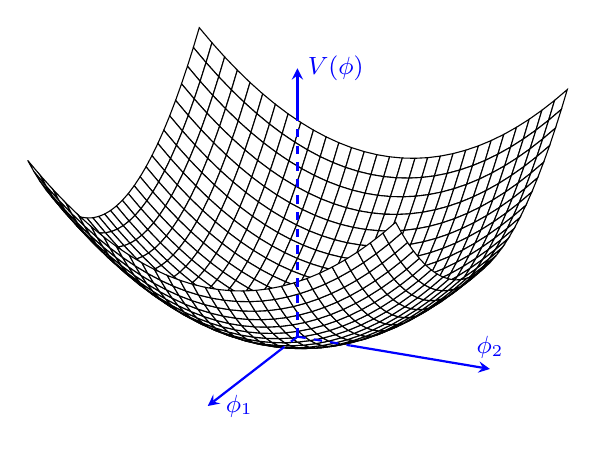
\begin{tikzpicture}%[scale=0.85]
    \begin{axis}[
        hide axis,
        %axis lines=middle,
        %            axis on top,
        %            axis line style={blue,dashed,thick},
        %            ymin=-2,ymax=2,
        %            xmin=-2,xmax=2,
        %            zmin=-2,zmax=2,
        samples=30,
        domain=-0.9:0.9,
        y domain=-0.9:0.9,clip=false
      ]
      \addplot3 [surf, shader=flat, draw=black, fill=white, z buffer=sort]
      ({0.85*x},{0.85*y},{0.85*x^2+y^2});
      \draw[blue,thick,dashed] (axis cs:0,0,0) -- (axis cs:0.22,0,0);
      %node[below,font=\small]{$\phi_{\text{IM}}$};
      \draw[blue,thick,-stealth] (axis cs:0.22,0,0) -- (axis cs:0.8,0,0)
      node[above,font=\small]{$\phi_{2}$};
      \draw[blue,thick,dashed] (axis cs:0,0,0) -- (axis cs:0,-0.15,0);
      %node[left=2mm,font=\small]{$\phi_{\text{RE}}$};
      \draw[blue,thick,-stealth] (axis cs:0,-0.15,0) -- (axis cs:0,-0.8,0)
      node[right=1mm,font=\small]{$\phi_{1}$};
      \draw[blue,thick,dashed] (axis cs:0,0,0) -- (axis cs:0,0,1.55);
      \draw[blue,thick,-stealth] (axis cs:0,0,1.55) -- (axis cs:0,0,1.9)
      node[right,font=\small]{$V(\phi)$};
    \end{axis}
  \end{tikzpicture}}
  \hspace{15mm}
  \subfloat[]{
  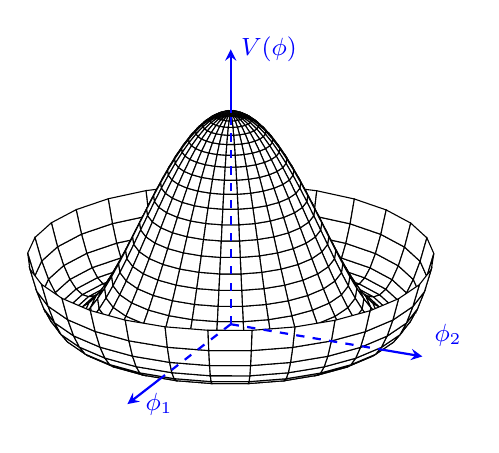
\begin{tikzpicture}
    \begin{axis}[
        hide axis,
        %axis lines=middle,
        %            axis on top,
        %            axis line style={blue,dashed,thick},
        %            ymin=-2,ymax=2,
        %            xmin=-2,xmax=2,
        %            zmin=-2,zmax=2,
        samples=30,
        domain=0:360,
        y domain=0:1.25,clip=false
      ]
      \addplot3 [surf, shader=flat, draw=black, fill=white, z buffer=sort]
      ({sin(x)*y}, {cos(x)*y}, {(y^2-1)^2});
      \draw[blue,thick,dashed] (axis cs:0,0,0) -- (axis cs:1,0,0);
      %node[below,font=\small]{$\phi_{\text{IM}}$};
      \draw[blue,thick,-stealth] (axis cs:1,0,0) -- (axis cs:1.3,0,0)
      node[above,font=\small]{~~~~~~$\phi_{2}$};
      \draw[blue,thick,dashed] (axis cs:0,0,0) -- (axis cs:0,-1,0);
      %node[left=2mm,font=\small]{$\phi_{\text{RE}}$};
      \draw[blue,thick,-stealth] (axis cs:0,-1,0) -- (axis cs:0,-1.5,0)
      node[right=1mm,font=\small]{$\phi_{1}$};
      \draw[blue,thick,dashed] (axis cs:0,0,0) -- (axis cs:0,0,1)
      %node[left=2mm,font=\small]{$\phi_{\text{RE}}$}
      ;
      \draw[blue,thick,-stealth] (axis cs:0,0,1) -- (axis cs:0,0,1.3)
      node[right,font=\small]{$V(\phi)$};
    \end{axis}
  \end{tikzpicture}}
  \caption{The Higgs potential in its fully and broken symmetric forms.}
  \label{fig:higgs-pot-01}
\end{figure}
 To suggest that
in our universe this symmetry is spontaneously broken is to suggest that the
values of these parameters evolved over time from the full to the broken state.
This ends up leading to masses for the vector bosons that are dependent on
$\mu^2$.

\section{Higgs Bosons at the LHC}
%
Higgs bosons are produced at the LHC in a number of different ways, the four
most common of which are shown in figure~\ref{fig:feyn-higgs-prod}.
\begin{figure}[ht]
  \centering
  \subfloat[]{
    \feynmandiagram [horizontal=a to b, yscale=0.9, xscale=0.8] {
      i1 [particle=\(g\)] -- [gluon] d -- [fermion, edge label=\(t\)] c -- [gluon] i2 [particle=\(g\)],
      i1 -- [draw=none] i2, 
      d -- [anti fermion, edge label=\(t\)] a -- [anti fermion, edge label=\(\overline{t}\)] c,
      a -- [scalar] b [particle=\(H^{0}\)],
    };
  }
  %\hspace{5.5mm}
  \subfloat[]{
    \feynmandiagram [horizontal=s to b, yscale=0.675, xscale=0.9] {
      i1 [particle=\(q_{1}\)] -- w1 -- f1 [particle=\(q_{2}\)],
      i2 [particle=\(q_{3}\)] -- w2 -- f2 [particle=\(q_{4}\)],
      s -- [draw=none] a,
      i1 -- [draw=none] s -- [draw=none] i2,
      w2 -- [photon] a -- [photon] w1,
      f1 -- [draw=none] b -- [draw=none] f2,
      a -- [scalar, edge label=\(H^{0}\)] b,
    };
  }
  %\vspace{1mm}
  \subfloat[]{
    \feynmandiagram [horizontal=a to b, scale =0.9] {
      i1 [particle=\(q\)] -- [fermion] a -- [fermion] i2 [particle=\(\overline{q}\)],
      a -- [photon, edge label=\(V\)] b,
      f1 [particle=\(V\)] -- [photon] b -- [scalar] f2 [particle=\(H^{0}\)],
    };
  }
  %\hspace{15mm}
  \subfloat[]{
    \feynmandiagram [horizontal=s to b, yscale=0.675, xscale=0.9] {
      i1 [particle=\(g\)] -- [gluon] q1 -- [anti fermion] f1 [particle=\(\overline{t}\)],
      i2 [particle=\(g\)] -- [gluon] q2 -- [fermion] f2 [particle=\(t\)],
      s -- [draw=none] a,
      i1 -- [draw=none] s -- [draw=none] i2,
      q2 -- a -- q1,
      f1 -- [draw=none] b -- [draw=none] f2,
      a -- [scalar, edge label=\(H^{0}\)] b,
    };
  }
  \caption{The four most common Higgs boson production methods from proton-proton collisions at the LHC.}
  \label{fig:feyn-higgs-prod}
\end{figure}
 The prevalence of these processes with
respect to the centre of mass energy of the proton-proton collision is shown in
figure~\ref{fig:higgs-br} (a). It can be seen the gluon-gluon fusion
(fig~\ref{fig:feyn-higgs-prod}~a) is by far the dominate contributor occurring
over an order of magnitude more than the next highest process which is quark
associated production (fig~\ref{fig:feyn-higgs-prod}~b). The next highest
production channel with respect to cross section is vector boson associated
(fig~\ref{fig:feyn-higgs-prod}~c) which will be the focus of the rest of this
report. Finally top quark associated production
(fig~\ref{fig:feyn-higgs-prod}~d) has the smallest cross section of these
processes.  The Higgs boson is predicted by the Standard Model to decay in a
number of different ways depending on its mass, a free parameter of the model.
In figure~\ref{fig:higgs-br} (b) the branching ratios of the Higgs can be seen,
plotted with respect to Higgs mass. The decay that will be focused on for the
rest of this report is $H~\rightarrow~b\bar{b}$.
\begin{figure}[ht]
  \centering
  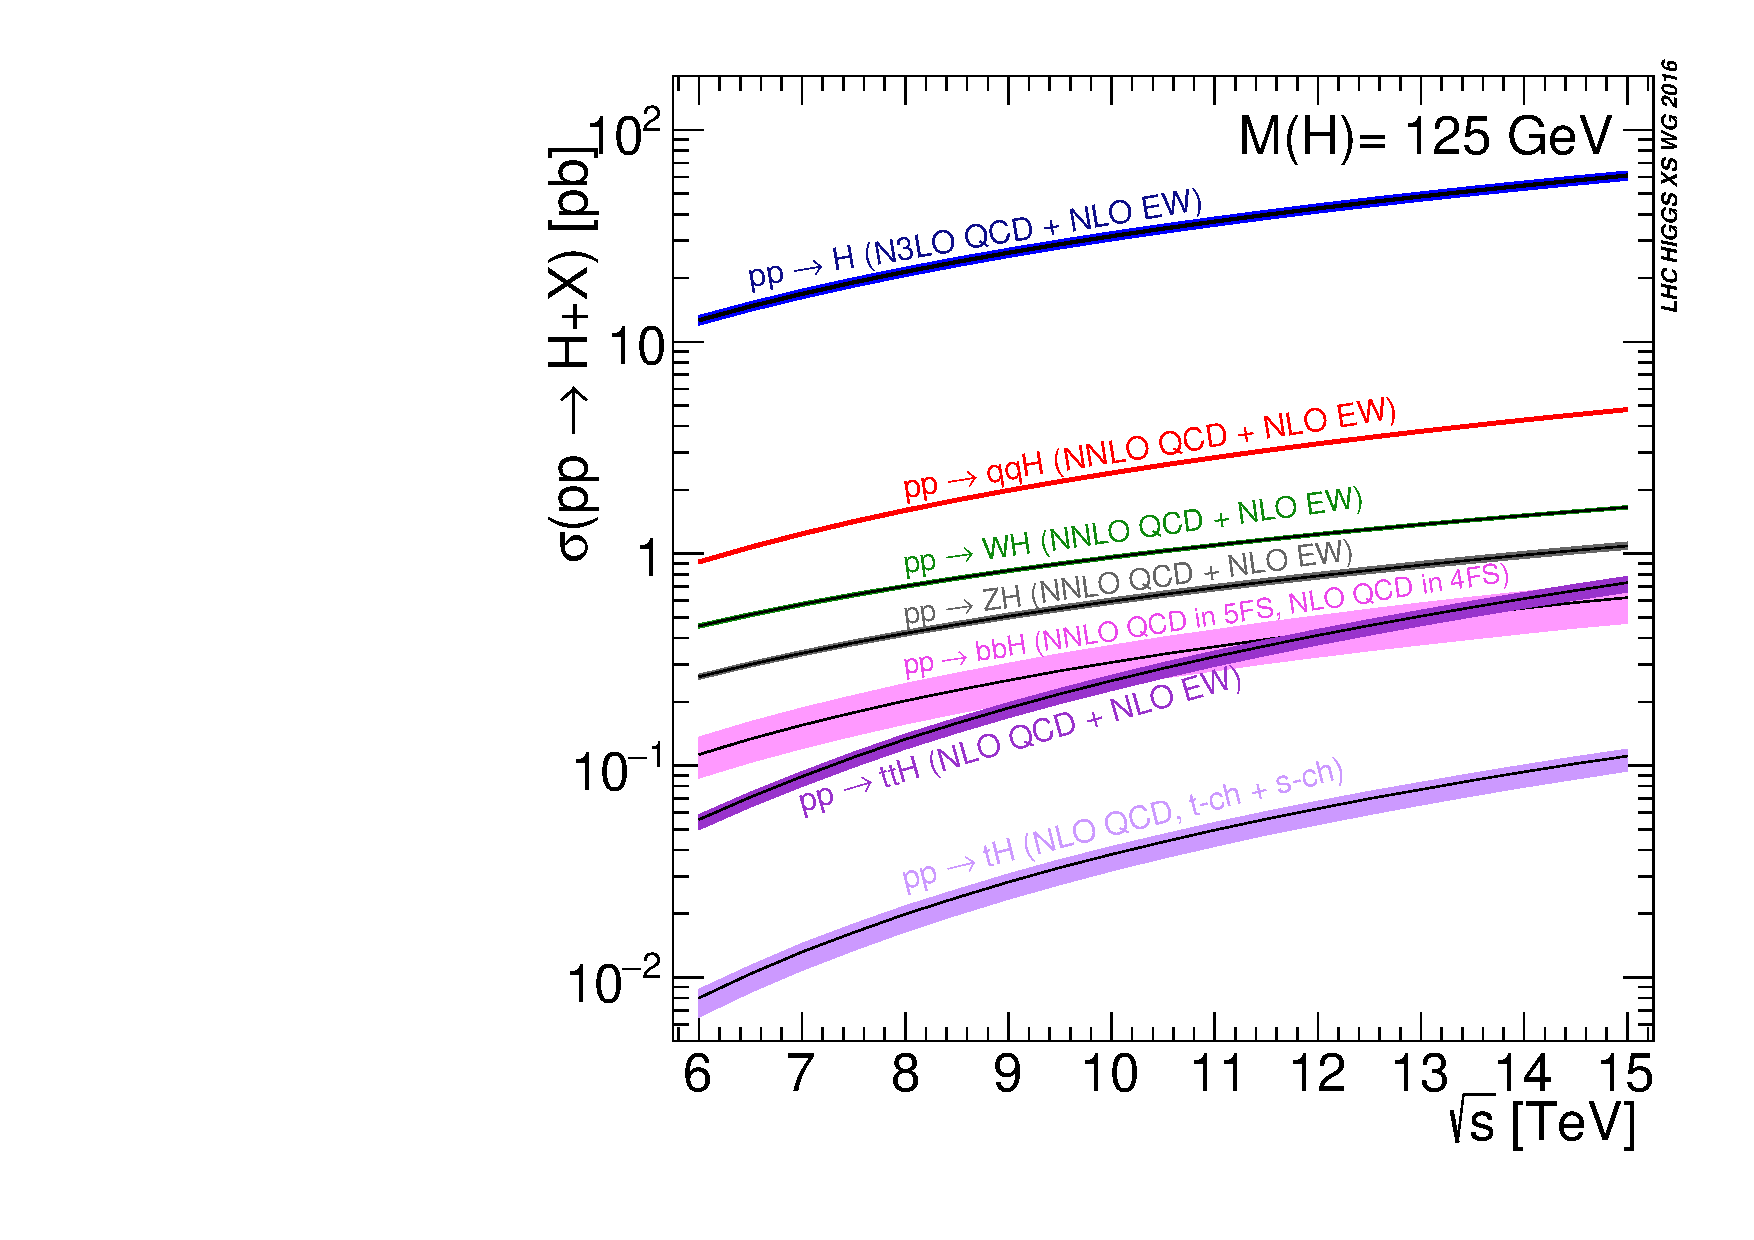
\includegraphics[width=.45\textwidth]{Plot_Escan_H125_xsec}%
  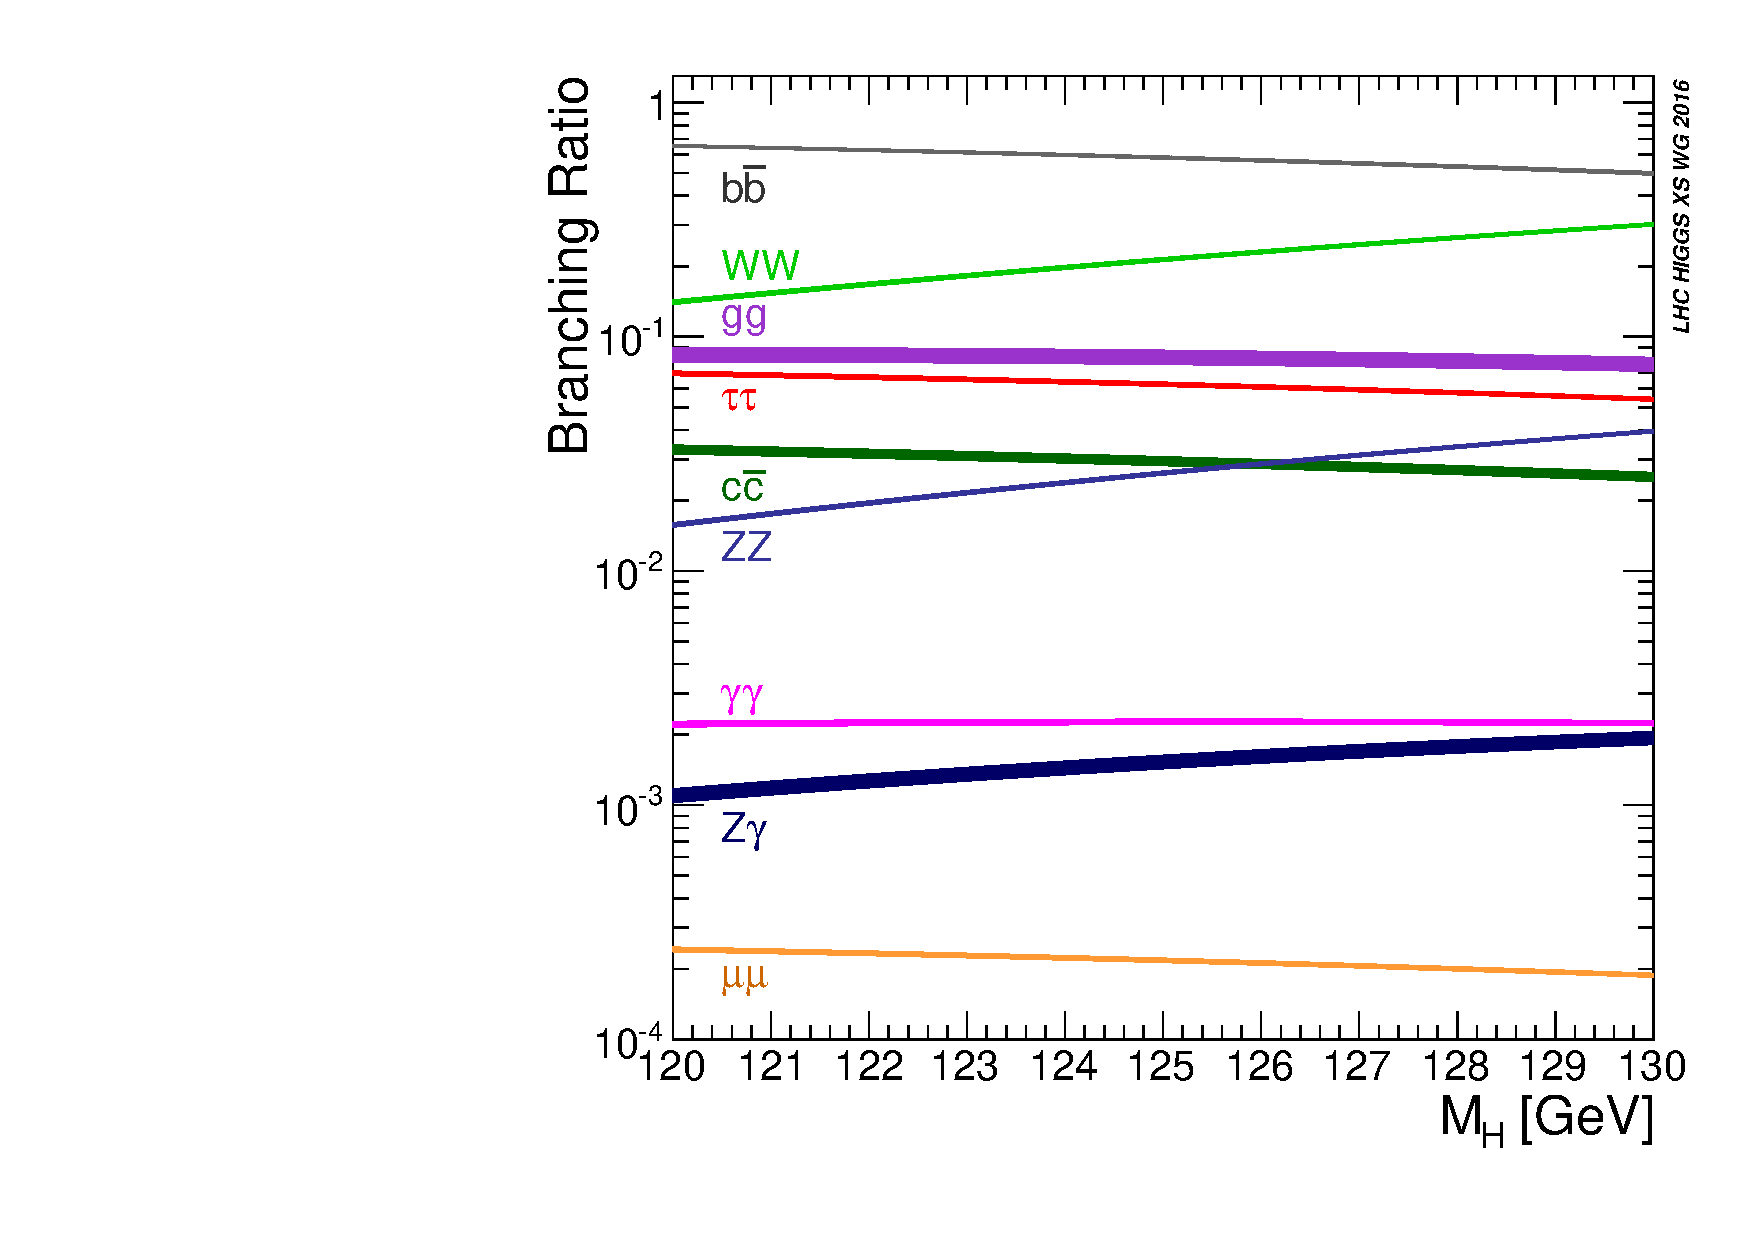
\includegraphics[width=.45\textwidth]{HiggsBR_mhscan}

  \caption[Higgs boson production cross sections and branching ratios.]{Higgs
    boson production cross-sections (left), and branching ratios (right) for a
    range of centre of meass energies and Higgs boson masses
    respectively~\cite{CERN-yellow-4}.}%
  \label{fig:higgs-br}
\end{figure}%
Given that the focus here is on vector boson associated production of a Higgs
boson it is also important to consider the decay of the vector boson. Three
possible scenarios are represented in figure~\ref{fig:feyn-vhbb}, namely the
situations where the vector boson decays to 1, 2 or 3 charged leptons and the
appropriate number of neutrinos. \begin{figure}
  \centering
  \feynmandiagram [horizontal=a to f] {
    i1 [particle=\(q\)] -- [fermion] a -- [fermion] i2 [particle=\(\overline{q}\)],
    a -- [photon, edge label=\(V\)] b -- [draw=none] f,
    w1 -- [photon, edge label=\(V\)] b -- [scalar, edge label=\(H^{0}\)] h1,
    l [particle=\(\ell^{+}/\overline{\nu}\)] -- [fermion] w1 -- [fermion] nu [particle=\(\ell^{-}/\nu\)],
    b1 [particle=\(\overline{b}\)] -- [fermion] h1 -- [fermion] b2 [particle=\(b\)],
    b2 -- [draw=none] f -- [draw=none] nu,
    h1 -- [draw=none] f -- [draw=none] w1,
  };
  \caption{A diagram showing a Higgs boson (decaying to a pair of b quarks) produced in association with a vector
    boson (decaying to 0, 1, or 2 charged leptons denoted $\ell^{+/-}$).
  }
  \label{fig:feyn-vhbb}
\end{figure}
 It is in fact
these leptonic decay modes that motivate the reason for studying this production
mechanism as opposed to one of the more common ones. The issue with looking at
the other production modes is that very large QCD generated backgrounds are
present due to initial state radiation. Whilst these backgrounds are also
present when looking at the vector associated channel they can be partially
suppressed by triggering on a lepton.
